%摘要
\section*{概述}
在整个数理逻辑课程的学习中,我在课堂上经常跟不上节奏,尤其是进入一阶逻辑的学习之后,我发现内容变得更加抽象,很难理解书本上抽象的定理和证明. 所以借这篇读书报告的机会,我反复阅读了一阶逻辑书本的内容,使用我觉得更加具象的方法表达我对书本内容的理解,思考了一些我自己感兴趣的点,结合书本上的一些题目,以及我做作业时没有搞明白的题目来完成这篇读书报告.

%介绍
\section{一阶逻辑和命题逻辑}
一阶逻辑和命题逻辑很显著的区别,便是引入了量词、谓词和变量,用量词来量化变量.

在命题逻辑中,原子也是一个命题,举一个命题逻辑中很简单和合式公式:$A \rightarrow B $

在这个句子中,$A$和$B$都是命题符号,也是命题逻辑能表达的最小的粒度. 也就是说,命题符号只能表达句子之间的关系. 

而来到一阶逻辑中,描述的最小的粒度也从命题/句子,缩小到了变量. 例如书本上给出的例子:$ {\forall x (Hx \rightarrow Mx)}.$

在这里,$ \forall x$指的是域内任意一个变量. 我们将为此符号$H$指定翻译为“是人”,将$M$翻译为“是好人”.那么对于人类这个定义域,无论是$s, p, q$(张三、李四、王五),都被x所代表. 也就是说,任意的“一个人是人”,便能得出“这个人是好人”.

在命题逻辑中拿出相似的例子:$H \rightarrow M$,只能将$H$翻译为“张三是人”,将$M$翻译为“张三是好人”,无法将句子拆开.

在这个对比中,命题逻辑只能描述一个人,而一阶逻辑可以描述所有人(当然,也可以表示某一些人),从这里不难看出,一阶逻辑使用谓词、变量来取代命题逻辑中的原子命题,原子的尺度从更大的“命题”变成了更小的项,也让语义更加丰富,描述的内容可以更加泛化,拓展了命题逻辑.

\section{一阶语言}
书本从一阶语言开始,逐步带着我们探究一阶逻辑.
\subsection{等于符号}
书中提到,要给定一个一阶语言,一定要指明两点:1.等于符号是否出现;2.参数有哪些.

等于符号为何如此重要吸引力我的注意. 书中解释与其他二元谓词符号相比,等于符号是一个逻辑符号而非参数. 那这句话应该如何理解?这样的不同又怎么对一阶语言造成影响?

等于符号有着固定、普遍使用的逻辑含义,表示逻辑上的等价关系. 而这样特殊的逻辑性质也就意味着等于符号的含义是不依赖语境的.

将等于符号和另外一个二元谓词符号$“<”$来进行对比. $“<”$ 表示小于关系,但是在不同的语境中可以有不同的含义,这里举两个例子:

1. 数学中的小于关系,$P(5, 10)$ 表示“$5 < 10$”. 这里的$“<”$是数值的比较,数字5小于10.

2. 时间上的小于关系,$P(5:00, 10:00)$ 表示$“5:00 < 10:00”$. 这里的$“<”$是时间的先后顺序,5:00早于10:00.

这里可以看到,同一个谓词符号在不同的语境中有着不同的含义. 但是对于等于符号来说,在任何情形下,他都有着相同的含义. 例如,我们可以说$P(5, 5)$表示$“5 = 5”$,这在任何情形下都是对的,而在任何情形下,$“5 = 6”$都是错误的,对等于符号的理解不需要依赖情景或领域.

等于符号的引入使得能够在一阶语言中表达相等,引入等式,并且判断逻辑一致性,扩充了一阶语言的表达能力.

\subsection{自由变量}
书中给出了自由变量的递归定义. 从直观上理解,将合式公式用树表达出来. 如果一个变量$x$在树中某一个向上的路径中没有被$\forall$修饰,那就认为这个变量$x$是自由出现的.

为了更好地理解和感受自由变量,我将书中定义转化为迭代来判断自由变量. 由于书中给出的递归并不是一个尾递归,而定义自由变量的本质也是遍历合式公式这棵“树”,我便想到了使用栈,伪代码如下:


\begin{figure}[H]
  \centering
  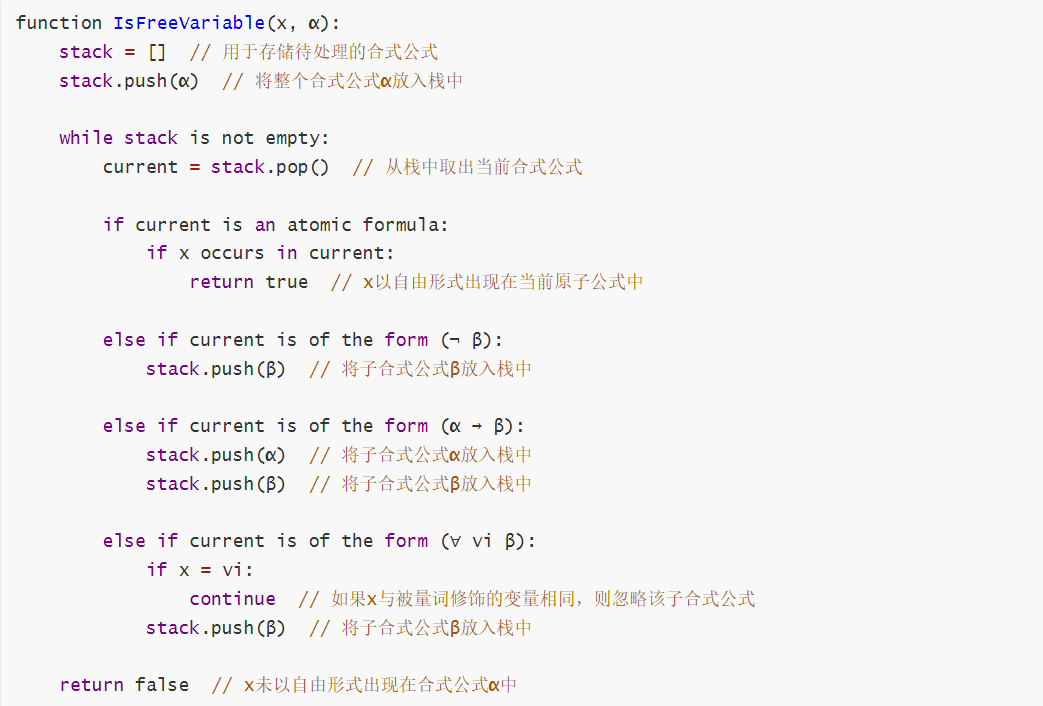
\includegraphics[width=\textwidth]{figure/2.png}
\end{figure}




习题2.1第九题

给出一个精确的定义说明:变量$x$在合式公式$\alpha$中作为第$i$个符号自由出现

这里通过类比书上对自由变量的递归定义,给出一个定义:

(1)对原子公式$\alpha$,变量$x$在$\alpha$中作为第$i$个符号自由出现当且仅当$x$在$\alpha$中作为第$i$个符号出现.

(2)$x$在$\neg \alpha$中作为第$i$个符号自由出现当且仅当$x$在$\alpha$中作为第$i - 1$个符号自由出现.

(3)$x$在$(\alpha \rightarrow \beta)$中作为第$i$个符号自由出现当且仅当$x$在$\alpha$中作为第$i - 1$个符号自由出现或者$x$在$\beta$中作为第$(i -len(a) - 2$个符号自由出现,$len(a)$表示$\alpha$的长度.

(4)$x$在$\forall v_1 \alpha$中作为第$i$个符号自由出现当且仅当$x$在$\alpha$中作为第$i - 2$个符号自由出现并且$x \neq v_1$.

\section{真值与模型}
\subsection{结构}
初读结构的定义,觉得很抽象难懂,也难以理解结构到底起到什么作用. 但是书上这一个例子一下打开了我的思绪:
\begin{figure}[H]
  \centering
  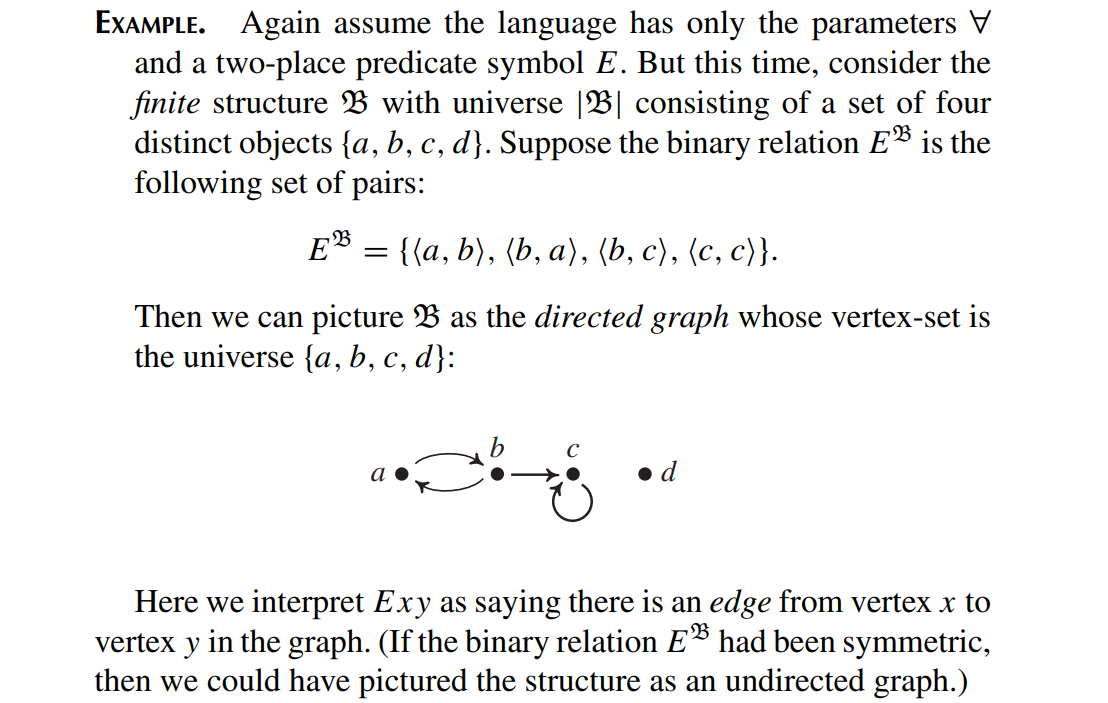
\includegraphics[width=\textwidth]{figure/1.png}
  \caption{}
  \label{}
\end{figure}

我意识到,在使用一阶语言时,并没有指定出量词所指的域是什么,也没有指出每个谓词符号应该如何解释. 正如上文我们提到,我们可以将" < "翻译成数值上的小于,也可以是时间上的早于. 也没有提到,哪些是我们可以比较的对象. 

考察$ {\forall}xPx$,这里我们可以有不同的理解

1. $x$的论域是\{1, 2, 3, 4, 5\},$Px$解释为$“x > 0”$

2. $x$的论域是南大学生,$Px$的解释是数学很好

   ...

在第一个解释中,$s$ 将 $x$ 映射到$\{1, 2, 3, 4, 5\}$中,并将$Px$ 映射为 $s(x) > 0$. 这样,就在一个论域为{1, 2, 3, 4, 5},$p$翻译为$“ > 0”$的结构上将合式公式翻译过来,使得合式公式有了具体的意义. 对于第二个例子而言,也是同样的. 一个简单的一阶语言合式公式,便可通过不同的的映射函数和结构获得完全不同的含义.

也就是说,一阶逻辑中的合式公式是抽象的,而通过函数$ s $以及其衍生出的 $\overline{s}$,将抽象的公式转化到结构中,赋予了合式公式具体的意义.

习题2.2 第三题 \{ $\forall x(\alpha \rightarrow \beta), \forall x\alpha \}\models \forall x\beta$.

第一眼看过去,这和假言推理很像,似乎很显然是对的,我在第一次做作业时也是这么想的. 但是当再次理解完一阶逻辑和结构时,我对这道题目有了不一样的看法. 在这里,出现了$\forall x$. 仅仅这一个合式公式并没有指明$\forall x$的域,更没有指明具体的结构. 所以这里的证明理应放到结构中去,证明应当是对于任意的结构和映射,和结构、映射本身的具体内容没有关系.

$\forall x(\alpha \rightarrow \beta), \forall x\alpha $

$\Rightarrow$对每一个结构 A 和映射函数 s: V→|A|,有 $\models_{A} \forall x(\alpha \rightarrow \beta)[s]$ 并且 $\models_{A} \forall x\alpha $[s]

$ \Rightarrow \forall d \in |A|,  \models_{A} \forall x(\alpha \rightarrow \beta)[s(x|d)]$ 并且 $\models_{A} \forall x\alpha [s(x|d)]$

$ \Rightarrow \forall d \in |A|, \models_{A} \forall x\alpha [s(x|d)]$ 并且 ($ \nvDash_{A} \forall x\alpha [s(x|d)]$或$\models_{A} \forall x\beta [s(x|d)]$)

$ \Rightarrow \forall d \in |A|, \models_{A} \forall x\alpha [s(x|d)]$ 

$ \Rightarrow \forall d \in |A|,\models_{A} \forall x\beta [s(x|d)]$

$ \Rightarrow \forall x\beta$

这道题目帮助我更好地理解了一阶逻辑与结构的关系.

\\ \hspace*{\fill} \\

习题2.2第十题

证明:$$\models_{A} \forall \nu_2 Q \nu_1 \nu_2[\![c^A]\!] \; iff. \; \models_{A} \forall \nu_2 Q c \nu_2$$

其中Q是二元谓词符号,c是常数符号.

$\models_{A} \forall \nu_2 Q \nu_1 \nu_2[\![c^A]\!]$

iff. 对每个s : V→|A|,有$ s(\nu_1) = c^A $ 并且$\models_{A} \forall \nu_2 Q \nu_1 \nu_2[\![s]\!]$

iff. 对每个s : V→|A|,有$ s(\nu_1) = c^A $ 并且对每个$d \in |A|$,有$\models_{A} Q \nu_1 \nu_2[\![s(\nu_2|d)]\!]$

iff. 对每个s : V→|A|,有$ s(\nu_1) = c^A $ 并且对每个$d \in |A|$,有$<s(\nu_1), d> \in Q$

iff. 对每个$d \in |A|$,有$<c^A, d> \in Q$

iff. 对每个$d \in |A|$,有$ \models_{A}Qcd$

iff. $\models_{A} \forall \nu_2 Q c \nu_2$

\section{演绎计算}
在解析算法之前,主要着重的是逻辑蕴含,这也是语义上的关系. 而来到演绎计算中,着重的是能够进行演绎,也就是通过公理或定理、规则能够在语法上证明出来.

我对这一章节的理解,就是通过六组公理以及规则T、概化定理、演绎定理等进行推理证明. 在这里我遇到的最大困难是不知道从何下手去进行证明,在这里梳理一下我一开始没有做出来,并且觉得很有意思的演绎和证明.

习题2.4 第三题

设A是结构,且令 s : V→|A|,在基本公式集上定义真值指派 v 如下:

$$ \nu (\alpha)=T   \; iff.  \; \models_{A}\alpha[s].$$

证明:对于任意公式(基本与否均可),有

$$ \overline{\nu} (\alpha)=T     \;   iff. \;  \models_{A}\alpha[s].$$

通过归纳进行证明

1. 对于基本公式 $\alpha$,$ \overline{\nu} (\alpha)=\nu (\alpha)=T$ iff.  $\models_{A} \alpha $[s].

2. $ \overline{\nu} (\neg\alpha)=T$ iff. $\nvDash_{A} \alpha $[s] iff. $\models_{A} \neg\alpha $[s].

3. $ \overline{\nu} (\alpha \rightarrow \beta)=T$

iff. $ \nu (\alpha)=F$ or $ \nu (\beta)=T$

iff. $\nvDash_{A} \alpha $[s] or $\models_{A} \beta $[s]

iff. $\nvDash_{A} \alpha \rightarrow \beta [s]$.

通过以上,可以归纳出$ \overline{\nu} (\alpha)=T     \;   iff. \;  \models_{A}\alpha[s].$

\\ \hspace*{\fill} \\

习题2.4 第四题

给出公式$\forall x \varphi \rightarrow \exists x \varphi$的(从$\emptyset$)的一个演绎.

公式$\forall x \varphi \rightarrow \exists x \varphi$毫无疑问是正确的,我们使用自然语言也可以很容易地说明. 但是如何使用给出演绎却着实难以下手.而通过几条基本公理、假言推理和规则T,最终很巧妙的得到了这样的一个演绎.

(1)$\forall x \emptyset \rightarrow \emptyset. \; Ax2.$

(2)$\forall x \neg \emptyset \rightarrow \neg \emptyset. \; Ax2.$

(3)$(\forall x \emptyset \rightarrow \emptyset) \rightarrow (\forall x \neg \emptyset \rightarrow \neg \emptyset) \rightarrow \forall x \emptyset \rightarrow \neg \forall x \neg \emptyset. \; T.$

(4)$(\forall x \neg \emptyset \rightarrow \neg \emptyset) \rightarrow \forall x \emptyset \rightarrow \neg \forall x \neg \emptyset. \; 1, 3; \; MP.$

(5)$\forall x \emptyset \rightarrow \neg \forall x \neg \emptyset. \; 2, 4; \; MP.$

(6)$\forall x \varphi \rightarrow \exists x \varphi.$

\\ \hspace*{\fill} \\

习题2.4 第十四题

证明:$$\vdash (\forall x((\neg Px) \rightarrow Qx) \rightarrow \forall y((\neg Qy) \rightarrow Py))$$

(1)$\vdash ((\neg Px) \rightarrow Qx) \rightarrow ((\neg Qx) \rightarrow Px). \; Ax1.$

(2)$\vdash \forall x[((\neg Px) \rightarrow Qx) \rightarrow ((\neg Qx) \rightarrow Px)]. \; 1; \; gen.$

(3)$\vdash \forall x[((\neg Px) \rightarrow Qx) \rightarrow ((\neg Qx) \rightarrow Px)]$ 

$\rightarrow \forall x((\neg Px) \rightarrow Qx) \rightarrow \forall x((\neg Qx) \rightarrow Px). \; Ax3.$

(4)$\vdash \forall x((\neg Px) \rightarrow Qx) \rightarrow \forall x((\neg Qx) \rightarrow Px). \; 2, 3; \;MP.$

(5)$ \forall x((\neg Px) \rightarrow Qx) \vdash \forall x((\neg Qx) \rightarrow Px). \; 4; \; MP.$

(6)$\vdash \forall x((\neg Qx) \rightarrow Px) \rightarrow ((\neg Qy) \rightarrow Py). \; Ax2.$

(7)$\forall x((\neg Px) \rightarrow Qx) \vdash ((\neg Qy) \rightarrow Py). \; 5, 6; \; MP.$

(8)$\forall x((\neg Px) \rightarrow Qx) \vdash \forall y((\neg Qy) \rightarrow Py). \; 7; \; G.$

(9)$\vdash (\forall x((\neg Px) \rightarrow Qx) \rightarrow \forall y((\neg Qy) \rightarrow Py)). \; 8; \; ded.$